% ****** Start of file apssamp.tex ******
%
%   This file is part of the APS files in the REVTeX 4.2 distribution.
%   Version 4.2a of REVTeX, December 2014
%
%   Copyright (c) 2014 The American Physical Society.
%
%   See the REVTeX 4 README file for restrictions and more information.
%
% TeX'ing this file requires that you have AMS-LaTeX 2.0 installed
% as well as the rest of the prerequisites for REVTeX 4.2
%
% See the REVTeX 4 README file
% It also requires running BibTeX. The commands are as follows:
%
%  1)  latex apssamp.tex
%  2)  bibtex apssamp
%  3)  latex apssamp.tex
%  4)  latex apssamp.tex
%
\documentclass[%
 reprint,
%superscriptaddress,
%grouhttps://www.overleaf.com/project/62e7efbe949d9b3fb167d1cdpedaddress,
%unsortedaddress,
%runinaddress,
%frontmatterverbose,
%preprint,
%preprintnumbers,
%nofootinbib,
%nobibnotes,
%bibnotes,
 amsmath,amssymb,
 aps,
%pra,
%prb,
%rmp,
%prstab,
%prstper,
%floatfix,
]{revtex4-2}

\usepackage{graphicx}% Include figure files
\usepackage{dcolumn}% Align table columns on decimal point
\usepackage{bm}% bold math
\usepackage{amsmath,amssymb,amsfonts}
\usepackage{algorithmic}
\usepackage{tabularx}
\usepackage{xcolor}
\usepackage{array}
    \newcolumntype{L}{>{\raggedright\arraybackslash}X}
\newcolumntype{P}[1]{>{\centering\arraybackslash}p{#1}}
\def\BibTeX{{\rm B\kern-.05em{\sc i\kern-.025em b}\kern-.08em
    T\kern-.1667em\lower.7ex\hbox{E}\kern-.125emX}}
%\usepackage{hyperref}% add hypertext capabilities
%\usepackage[mathlines]{lineno}% Enable numbering of text and display math
%\linenumbers\relax % Commence numbering lines

%\usepackage[showframe,%Uncomment any one of the following lines to test
%%scale=0.7, marginratio={1:1, 2:3}, ignoreall,% default settings
%%text={7in,10in},centering,
%%margin=1.5in,
%%total={6.5in,8.75in}, top=1.2in, left=0.9in, includefoot,
%%height=10in,a5paper,hmargin={3cm,0.8in},
%]{geometry}

\begin{document}

\preprint{APS/123-QED}

\title{Spurious Solar-Wind Effects on Acceleration Noise in LISA Pathfinder}% Force line breaks with \\
\author{Arnold Yang\(^1\)}%
\author{Indie Desiderio-Sloane\(^1\)}
 \author{Grant David Meadors\(^2\)}

\affiliation{%
Institute for Computing in Research\(^1\)
 Los Alamos National Laboratory\(^2\)
}%

\date{\today}% It is always \today, today,
             %  but any date may be explicitly specified

\begin{abstract}
Spurious solar wind effects may contribute as a candidate noise factor on the precise instrumentation of the future Laser Interferometer Space Antenna(LISA). To predict the possible impact of this noise factor, models were made to display spurious solar wind effects on acceleration noise in LISA Pathfinder. Data from NASA's Advanced Composition Explorer(ACE) which was also situated at the L1 Lagrange point was used as a reliable source of Solar Wind data. To test this, the data from both satellites was formatted, gap-filled and adapted for comparison and a coherence plot was created comparing the results of the fast Fourier transformations. The coherence plot suggested that Solar Wind had minuscule effect on the LPF and higher frequency coherence(LISA’s main observing band) can be attributed to random chance correlation. This is great news for the future LISA project as this suggests higher instrumentation accuracy and that solar wind is not a major source of noise.
\end{abstract}

%\keywords{Suggested keywords}%Use showkeys class option if keyword
                              %display desired
\maketitle

%\tableofcontents

\section{introduction}
The future Laser Interferometer Space Antenna(LISA) will be working towards looking back past the Cosmic Microwave Background and expanding on the work done by the Laser Interferometer Gravitational Wave Observatory(LIGO) by measuring gravitational waves. To test the LISA concept, an early satellite, the LISA Pathfinder(LPF), was sent up with similar equipment to the future LISA.  The LPF used 2 pure free-falling masses at which the accelerations at the femto-g level could be measured, the same level at which minute gravitational wave passes can be dtected[5]. To ensure reliability a control system was introduced to keep the test masses centered in the spacecraft[4]. With such precise instrumentation the control system is designed to counteract a multitude of disturbances including solar wind/irradiance, micrometeoroids, and gravity from other interstellar mass. The LPF flew no instrumentation to measure the spurious solar wind effect. Therefore using current solar wind satellite the Advanced Composition Explorer(ACE), various plots were made comparing 1,684 hours of LPF and ACE data across a 3 and a half month time span to estimate the effects of solar wind on the LISA.

Solar wind originates from coronal mass ejections made by disturbances in the Sun’s corona. The emitted high speed charged particles can reach speeds of 1 million miles per hour, larger storms have been known to be damaging to satellite function and are causes for inaccuracy of GPS satellites. The charges of these particles have a lesser effect on the LPF satellite as its instruments measure the acceleration of 2 free-falling masses. However, solar wind may contribute to a small force on the movement of this mass which contributes to regular noise in the data. This paper will detail the necessary steps to format, transform, and plot data from ACE and LPF. Then the paper will discuss the results and the conclusion reached via the results.

\subsection{\label{sec:level2}Related Works}
Spatial weather has been identified as a key noise factor in possible future LISA measurements. Past work in assessing the impact involved using SOHOs Virgo Solar irradiance and ACE Solar Wind data to model possible impacts on the future LISA space antenna(Frank et al. 2020). [1] Another major source of noise identified for LPF is micrometeoroids[4]. Through processing the whole LPF data, 54 impact candidates were identified and were shown to be similar to those resulting from Jupiter Family Comets(JFC), Oort cloud comets, Halley-type comets, and asteroids. Additionally, the creation of LISA is renewing the interest in the environment of space. This environment includes solar energetic particles, galactic cosmic ray fluxes, and the effects of solar neutrons and interplanetary electrons[2].

\section{Methods}
This section describes the steps taken to format, compile, and plot data from ACE and LPF.
\begin{figure}[htbp]
\centerline{
\includegraphics[width=0.5\textwidth]{fig1solWmam.jpg}}
\caption{Flow diagram for steps taken}
\label{fig}
\end{figure}
\subsection{ACE data-Formatting, Filtering, Gap Filling, Calculations
}
We used solar wind data from the Advanced Composition Explorer(ACE), which provided solar wind velocity components, alpha particle to proton ratios, proton densities at 64 second intervals measured in UTC time[3]. Further formatting required converting UTC time to the GPS time format used by LPF data and filtering and gap filling all bad data values(-9999.9 as specified in the ACE data file header)[3]. The gaps were separated into 3 categories by length using the method of gap fill from \textit{Modeling Spurious Forces on the LISA Spacecraft Across a Full Solar Cycle} [1], for best effect when Fourier transformation is used. Type A gaps are of length 1 and can be filled with simple linear interpolation (averaging values on either side of the graph). Type B gaps are of lengths between 2 and 24 and filled with a combination of Gaussian Noise and linear interpolation. For the Gaussian noise(\(\sigma\)) to have similar characteristic to the data around it, \(sigma_{1}\) and \(\sigma_{2}\) are the standard deviations sampling data of equal length to the gap on either side of the gap[1].

\begin{equation}\label{eq:Gaussian Window Equations}
\sigma=\frac{l-(i-1)}{l+1}\sigma_{1}+\frac{i}{l+1}\sigma_{2}
\end{equation}

For Type C gaps of lengths greater than or equal to 25, Gaussian Noise may introduce unnecessary noise, thus a Hanning Window is used, with a slow falloff to 0 to fill the gaps[1]. These gaps use 25 data point from before the gap and 25 data points after the gap to run Eqs. (2).
%\;\;\;\;\;(1)

\begin{equation}\label{eq:Hanning Window}
\omega(n)=0.5[1-\cos{(\frac{2\pi n}{N-1})}]
\end{equation}
where \textit{N}=51 and 0$<$\textit{n}$>$\textit{N}-1

\begin{table}[htbp]
\caption{Gap fill methods by length}
\begin{center}
\renewcommand{\arraystretch}{1.5}
\begin{tabular}{|c|c|c|}
\hline
%\textbf{Table}&\multicolumn{3}{|c|}{\textbf{Table Column Head}} \\
Type & Length & Fill Method\\
%\textbf{Head} & \textbf{\textit{Table column subhead}}& \textbf{\textit{Subhead}}& \textbf{\textit{Subhead}} \\
\hline
A & 1 & Linear Interpolation\\
\hline
B & 2-24 & Gaussian Noise with Linear Interpolation\\
\hline
C & $\geq$25 & Hann Window\\
\hline
%copy& More table copy$^{\mathrm{a}}$& &  \\

%\multicolumn{4}{l}
%\multicolumn{4}{l}{$^{\mathrm{a}}$P values were computed by the Mann-Whitney-U test.}
\end{tabular}
\label{tab1}
\end{center}
\end{table}



After all parts of the data are filtered and gaps are filled, the data in its raw form consists of 6 used components: solar wind velocity components(x, y, z), alpha particle to proton ratios, proton densities and proton speed at 64 second intervals. To simulate force data for comparison with the LISA Pathfinder, modeling equations from [1] are used. We start by calculating the number of particles per unit time colliding with the satellite Eqs. (3)[1].
\begin{equation}\label{eq:Hanning Window}
N=n v Acos(\phi),
\end{equation}
where n is particle density, v is wind speed, Acos(\(\phi\)) represents the surface area of the LPF satellite with A being the solar array area and \(\phi\) being the angle between the normal of the array and the orbital plane[1]. In our calculations \(\phi\) was approximated to 0.0349066 radians(2 degrees) as changes in it are minimal.

The force equations are as follows[1]:
\begin{equation}\label{eq:Hanning Window}
\begin{split}
F_{x}=(N_{p}m_{p}+N_{\alpha}m_{\alpha})[(1+Rcos(2\phi))v_{x}+Rsin(2\phi)v_{z}], \\ F_{y}=(N_{p}m_{p}+N_{\alpha}m_{\alpha})[(1-R)v_{y}], \\ F_{z}=(N_{p}m_{p}+N_{\alpha}m_{\alpha})[(1+Rcos(2\phi))v_{z}+Rsin(2\phi)v_{x}],
\end{split}
\end{equation}
 \(N_{p}\) and \(N_{\alpha}\) from Eqs. (3) are proton and alpha particle collision rates with the satellite, \(m_{p}\) and \(m_{\alpha}\) are proton and alpha particle mass respectively. \(v_{x},v_{y},v_{z}\) are the x,y,z components of solar wind velocity. Thereafter, assuming all particles are reflected(worst case scenario), Eqs. (4) are used to convert particle rate to Force, and the equation simplifies to Eqs. (5)[1].



%\(F_{x}=(N_{p}m_{p}+N_{\alpha}m_{\alpha})[(1+cos(2\phi))v_{x}+Rsin(2\phi)v_{z}]\),
%\(F_{y}=0\),
%\(F_{z}=(N_{p}m_{p}+N_{\alpha}m_{\alpha})[(1+cos(2\phi))v_{z}+Rsin(2\phi)v_{x}]\) (4)
%\begin{equation}
%\end{equation}
%\iffalse
\begin{equation}\label{eq:Hanning Window}
\begin{split}
F_{x}=(N_{p}m_{p}+N_{\alpha}m_{\alpha})[(1+cos(2\phi))v_{x}+sin(2\phi)v_{z}], \\ F_{y}=0, \\ F_{z}=(N_{p}m_{p}+N_{\alpha}m_{\alpha})[(1+cos(2\phi))v_{z}+sin(2\phi)v_{x}].
\end{split}
\end{equation}
%\fi

\subsection{LISA Pathfinder data-Formatting, Filtering. Gap Filling}
To estimate the effect of solar irradiance and solar wind on the future LISA space antenna, data from the LPF was used. Obtained from NASA Goddard, the data is calibrated to combine information on the various sensors, actuators, position controllers along with knowledge on altitude, and spacecraft mass properties to estimate effective free-body motion of the spacecraft[4]. 114 days worth of data taken at about 2.5 second intervals across 370 16384 second duration from the second sensor from the z-axis on the spacecraft was used. Data was received in having been run through a Fast Fourier Transformation and all values were positive non-zero frequencies. Therefore, 0s, positive non-zero frequencies and complex conjugates of negative frequencies were added to the data before taking an Inverse Fourier Transform to reconstruct the original time series. There were 30 gaps in the data and all gaps were filled with the Hanning window(TypeC) Eqs. (3) method mentioned in the ACE methods[1].

\subsection{Plotting and Analysis}
To compare the ACE to LISA data five types of plots were used as seen in Figures 2-6. \\
\begin{figure}[htbp]
\centerline{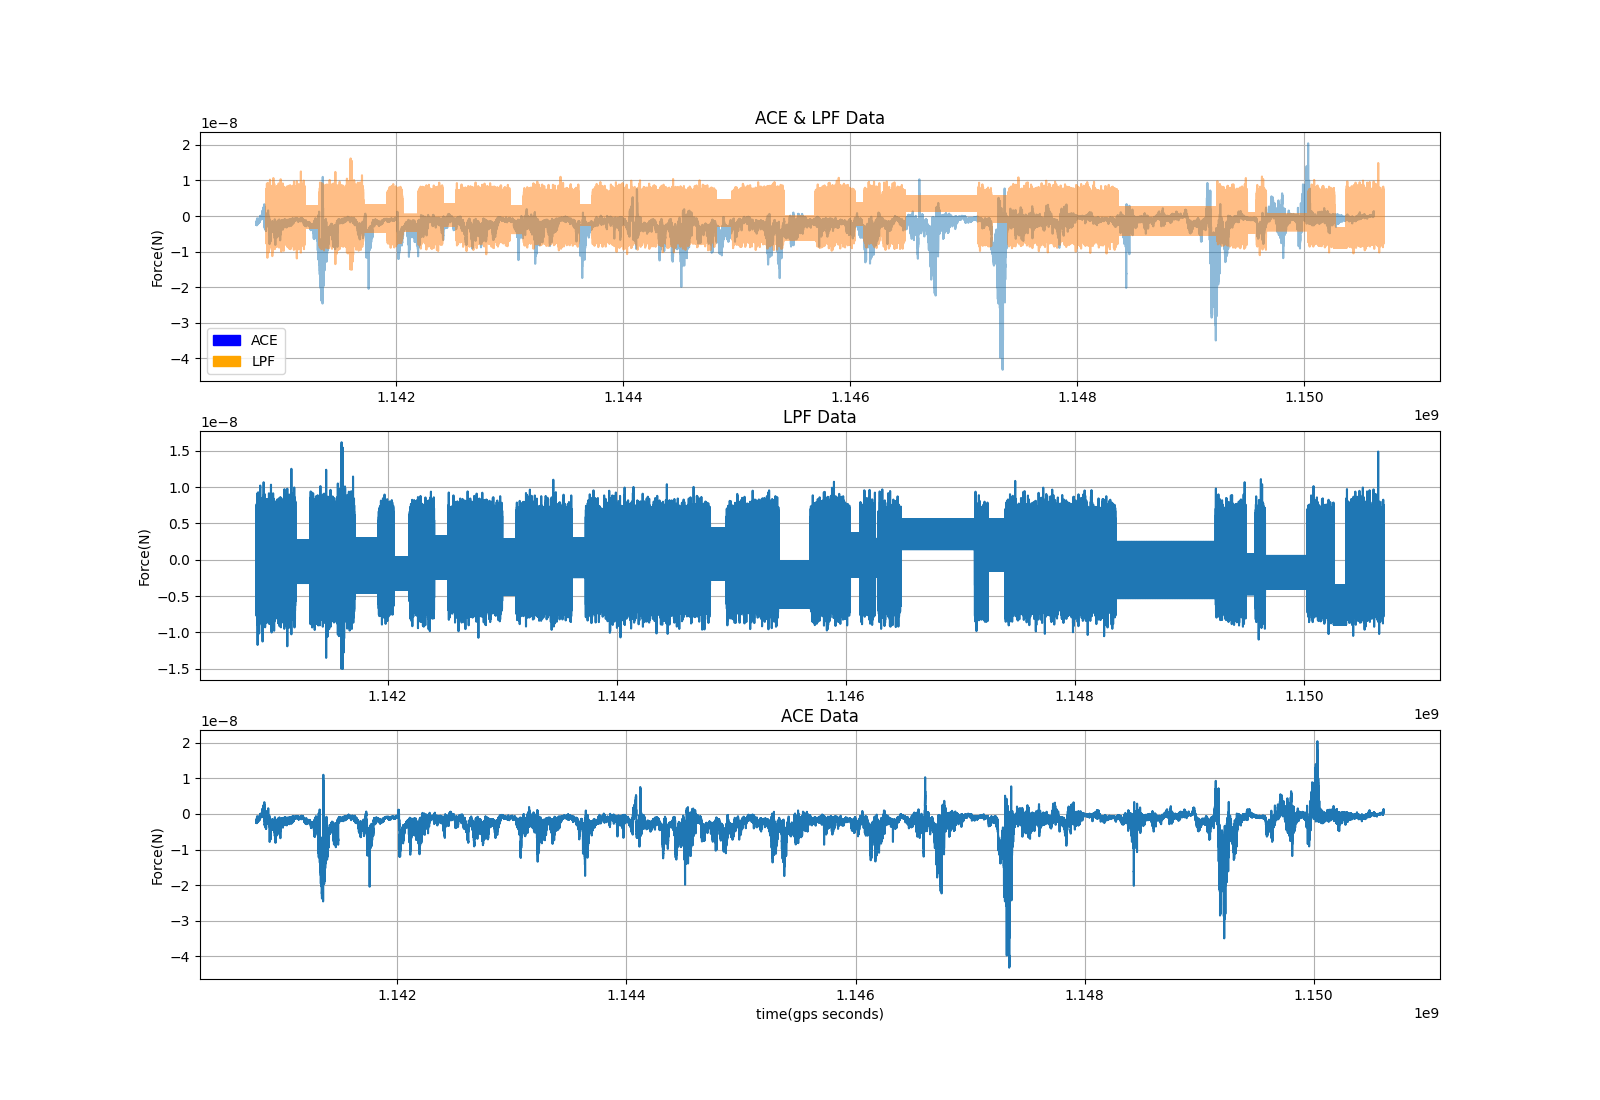
\includegraphics[width=0.5\textwidth]{TimeDomain_Comparison_ACEvLPF.png}}
\caption{Timesireis plot of ACE and LPF}
\label{fig}
\end{figure}
Figure 2 shows a normal direct time series comparison, showing what the 2 signals look like when graphed together and apart.\\
\begin{figure}[htbp]
\centerline{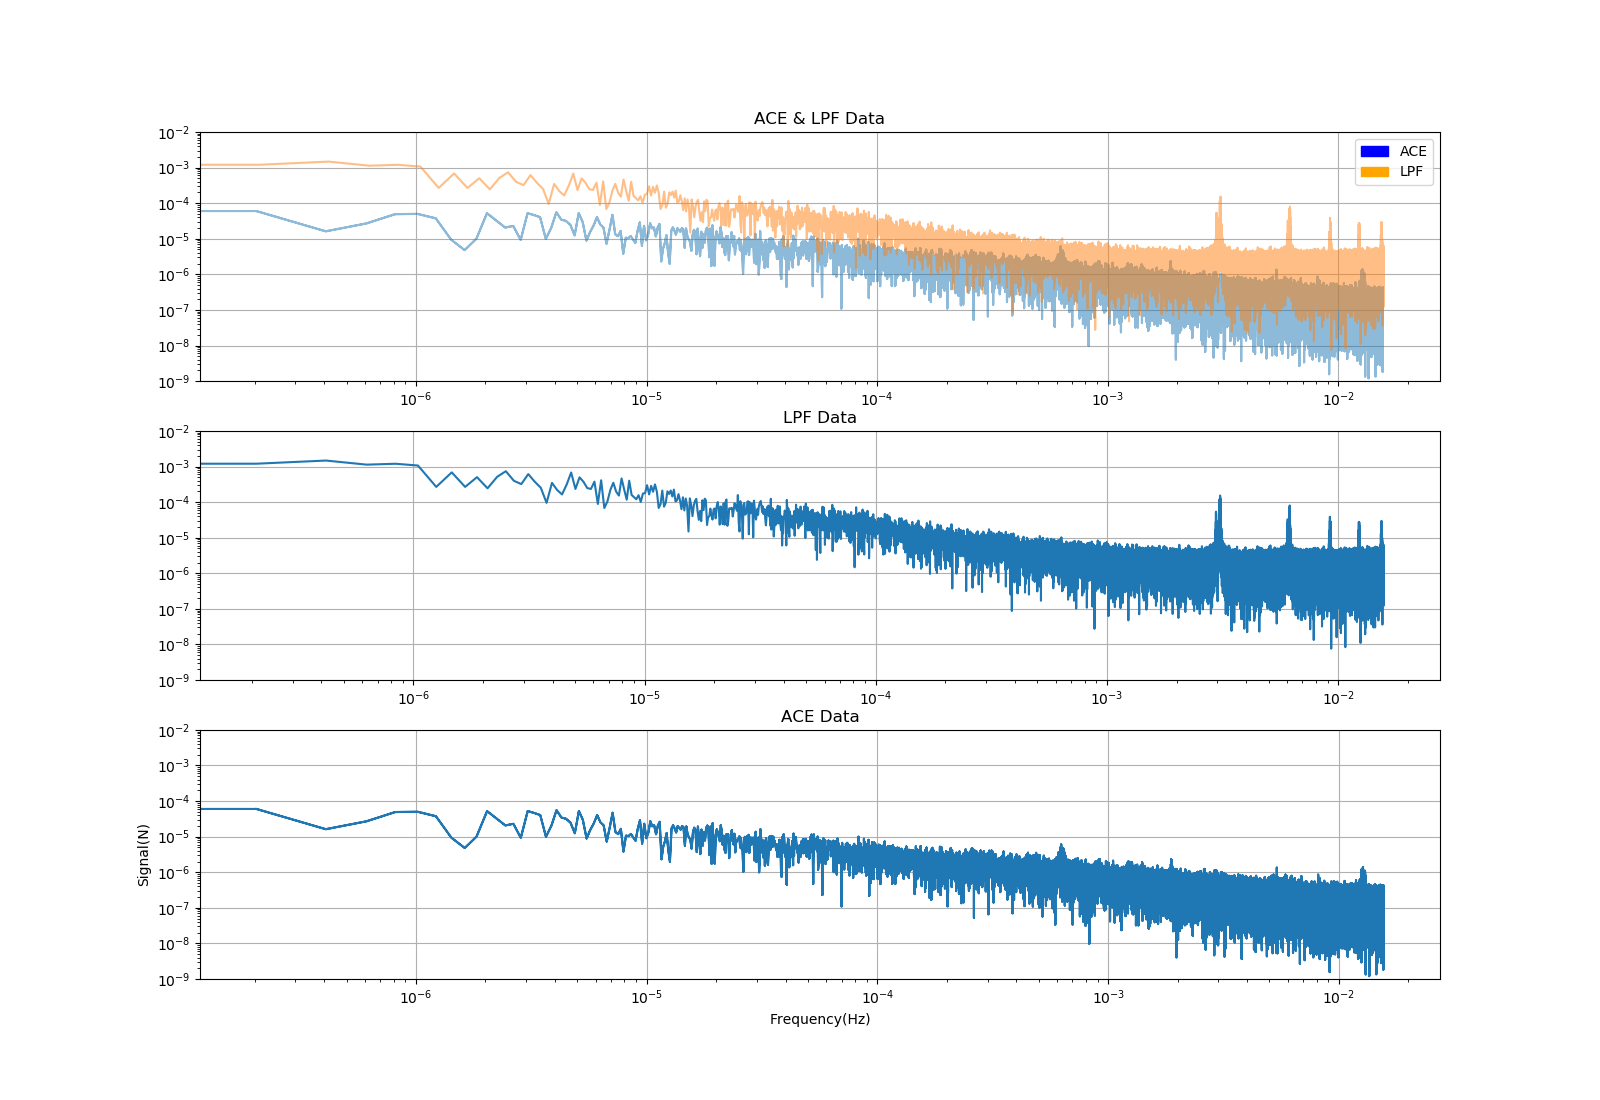
\includegraphics[width=0.5\textwidth]{ACE_and_LPF_Loglog.png}}
\caption{FFT plot of ACE and LPF on a loglog scale}
\label{fig}
\end{figure}
Figure 3 shows the amplitude spectrum of the Fast Fourier Transformation of the data, corresponding to similar signal frequencies between both graphs. Figure 2 truncates the higher frequencies of the Pathfinder data in the comparison, to directly match the lower frequencies that the ACE data has due to the lower sampling rate. Due to bad data, there are huge spikes in the data at the lowest frequencies, therefore, the graph uses a loglog scale.\\
\begin{figure}[htbp]
\centerline{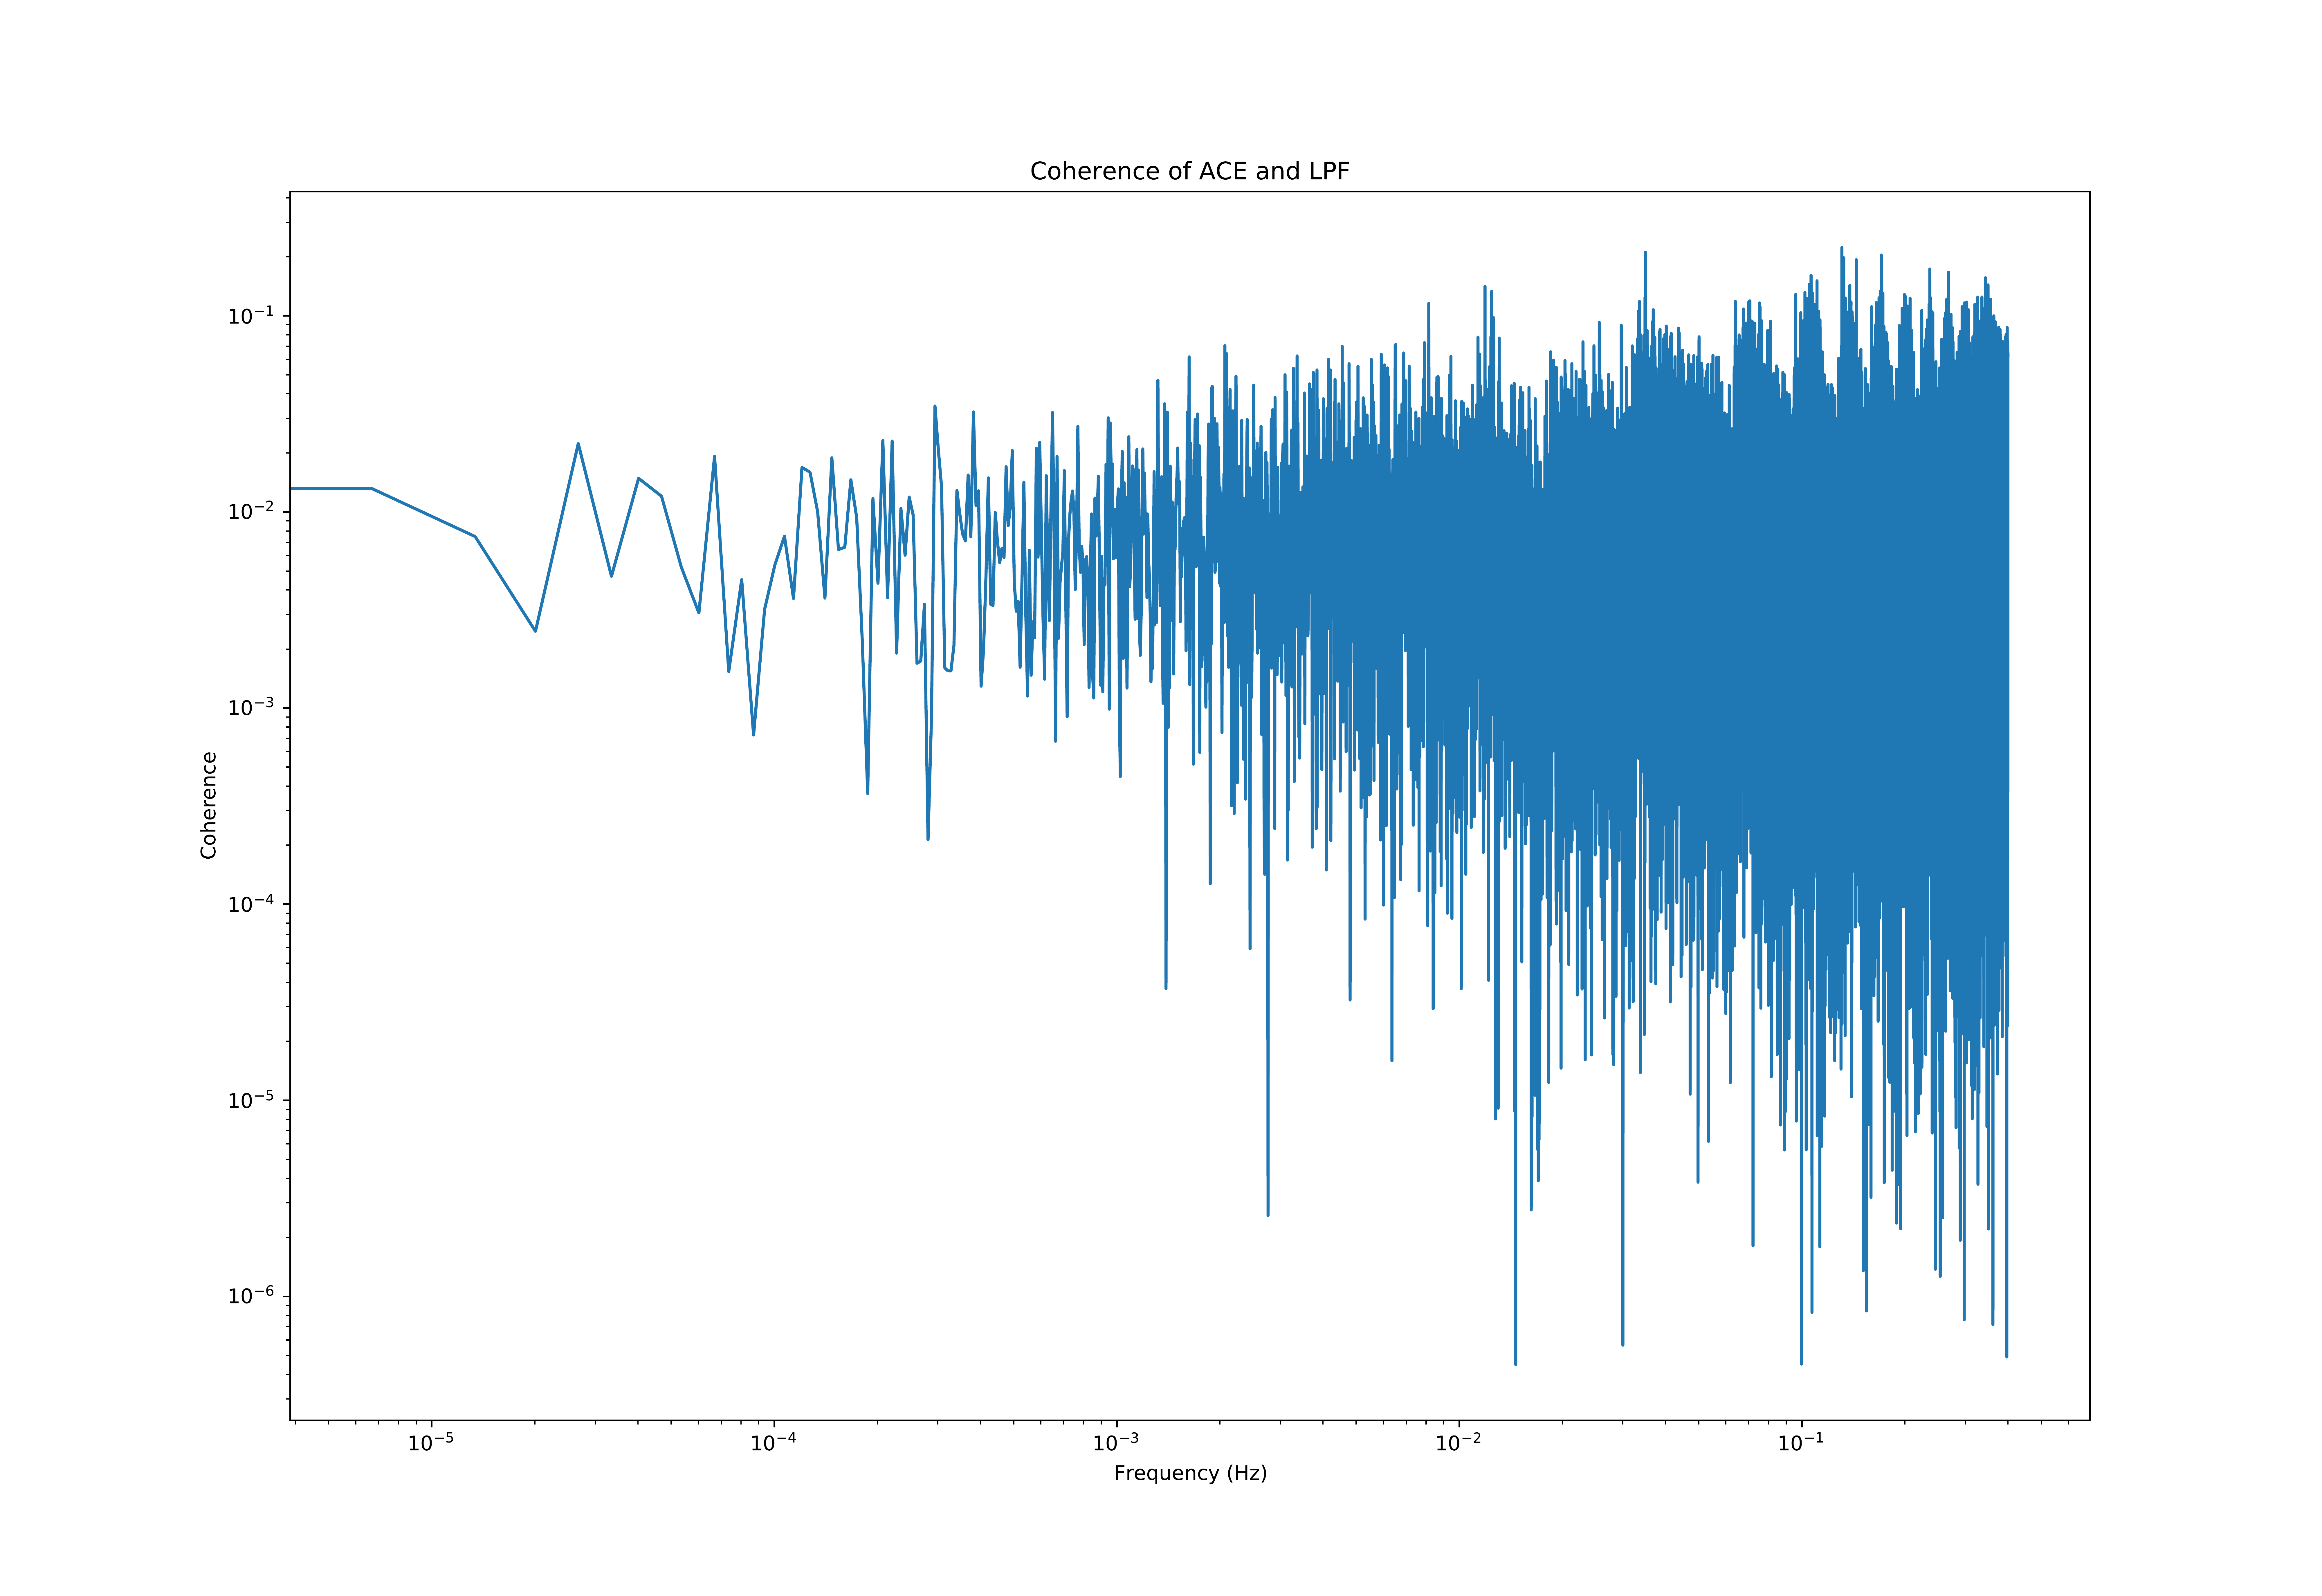
\includegraphics[width=0.5\textwidth]{ACE_and_LPF_co.png}}
\caption{Coherence plot of ACE and LPF}
\label{fig}
\end{figure}
Figure 4 is a coherence plot which shows how much the ACE and LPF data cohere to one another. A higher coherence value shows that the solar wind measured in the ACE data had some effect on the acceleration noise of the LPF data. A lower value displays a lack of correlation between the data values.\\
\begin{figure}[htbp]
\centerline{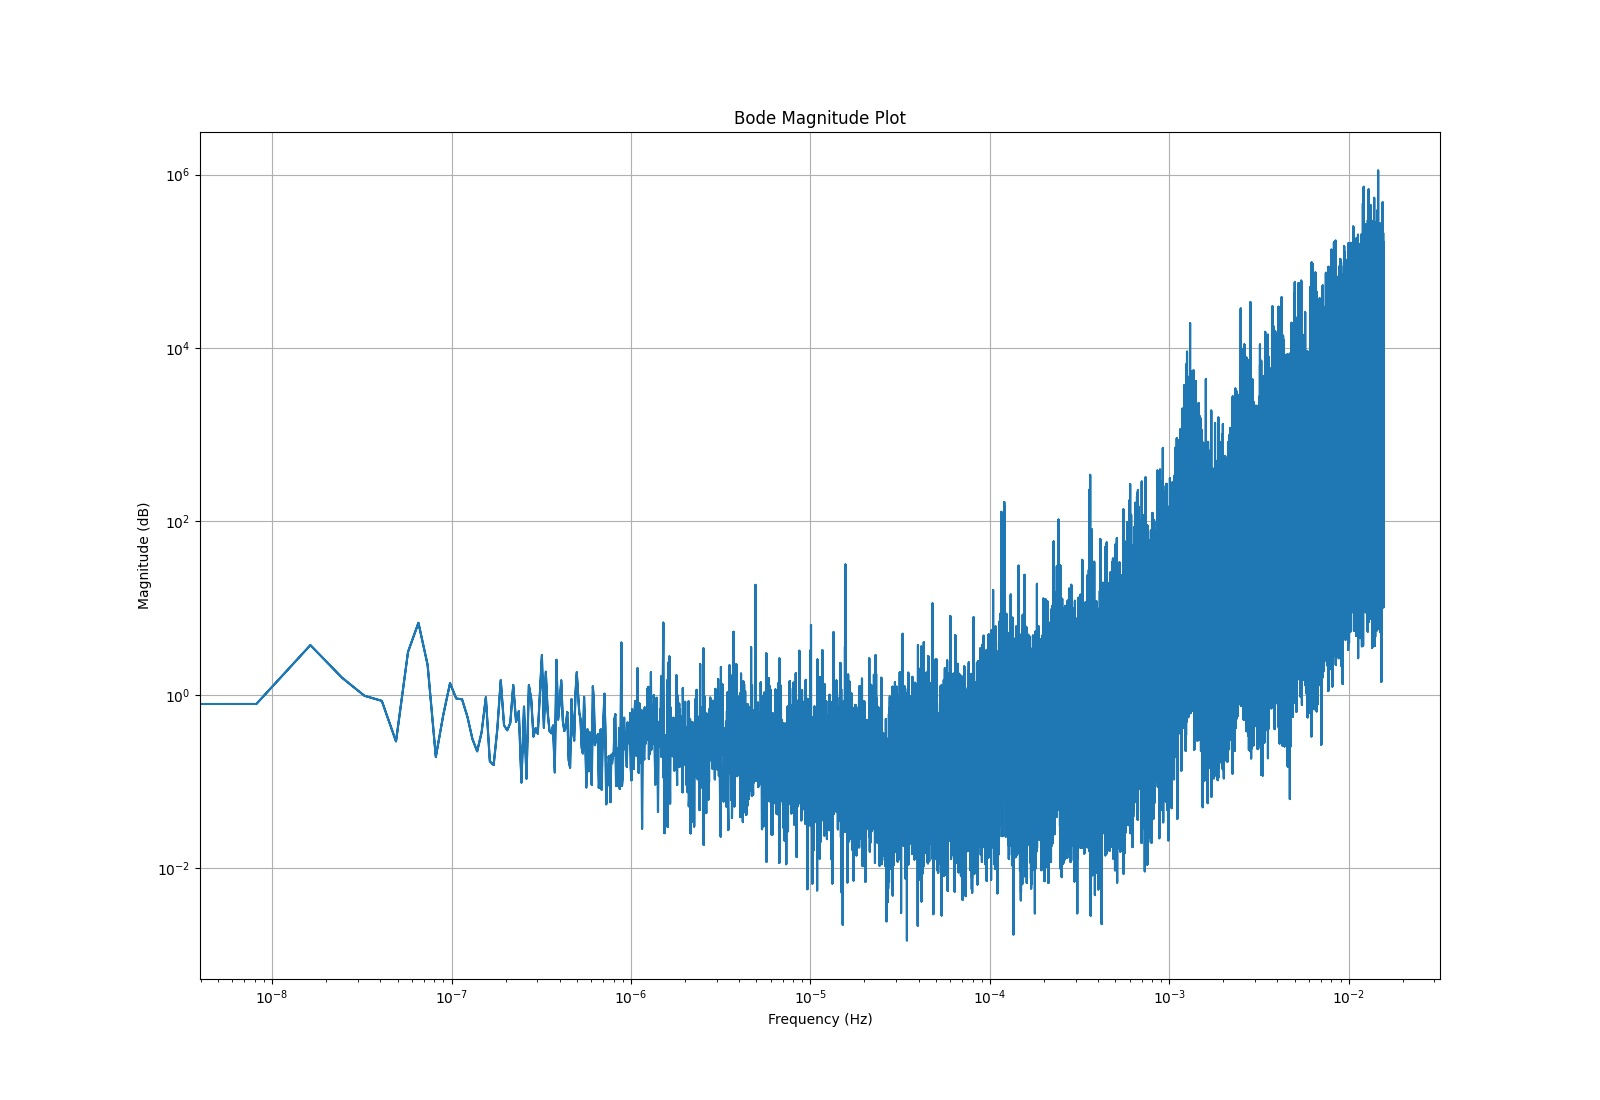
\includegraphics[width=0.5\textwidth]{Bode_Magnitude_Plot.jpg}}
\caption{Bode magnitude plot}
\label{fig}
\end{figure}
\begin{figure}[htbp]
\centerline{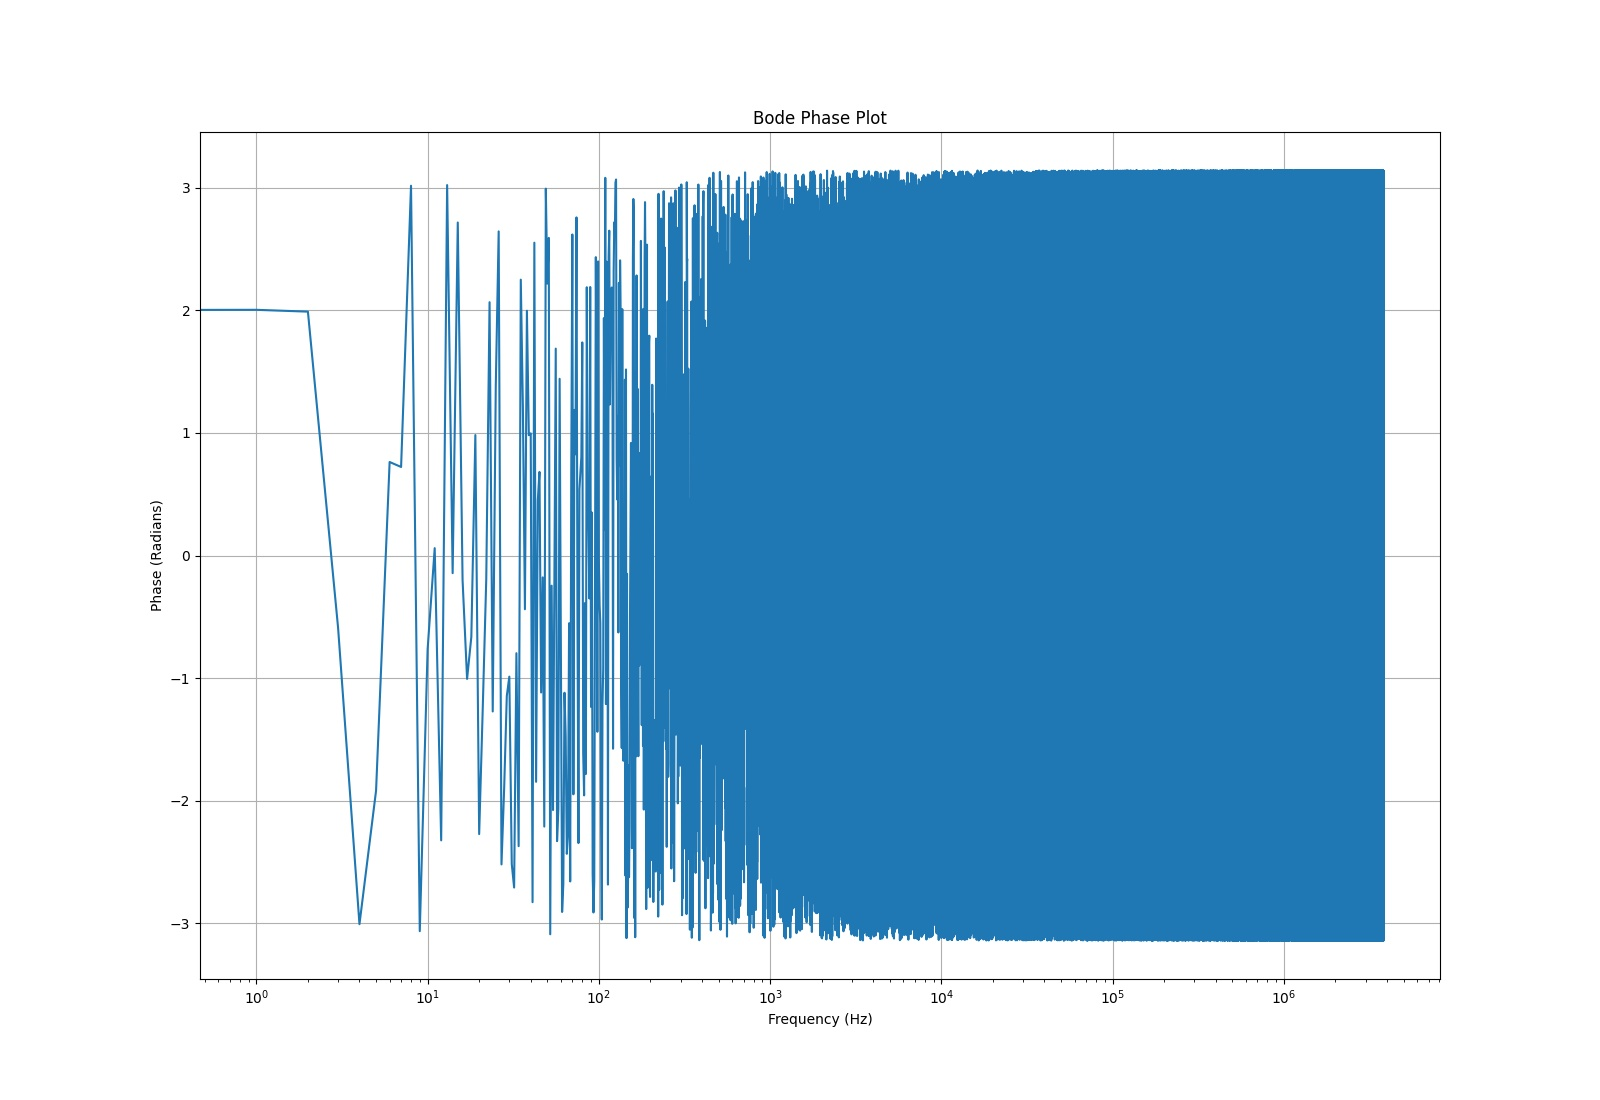
\includegraphics[width=0.5\textwidth]{Bode_Phase_Plot.jpg}}
\caption{Bode phase plot}
\label{fig}
\end{figure}
Figure 5 and 6 displays a Bode magnitude and a Bode phase plot. \\
\begin{figure}[htbp]
\centerline{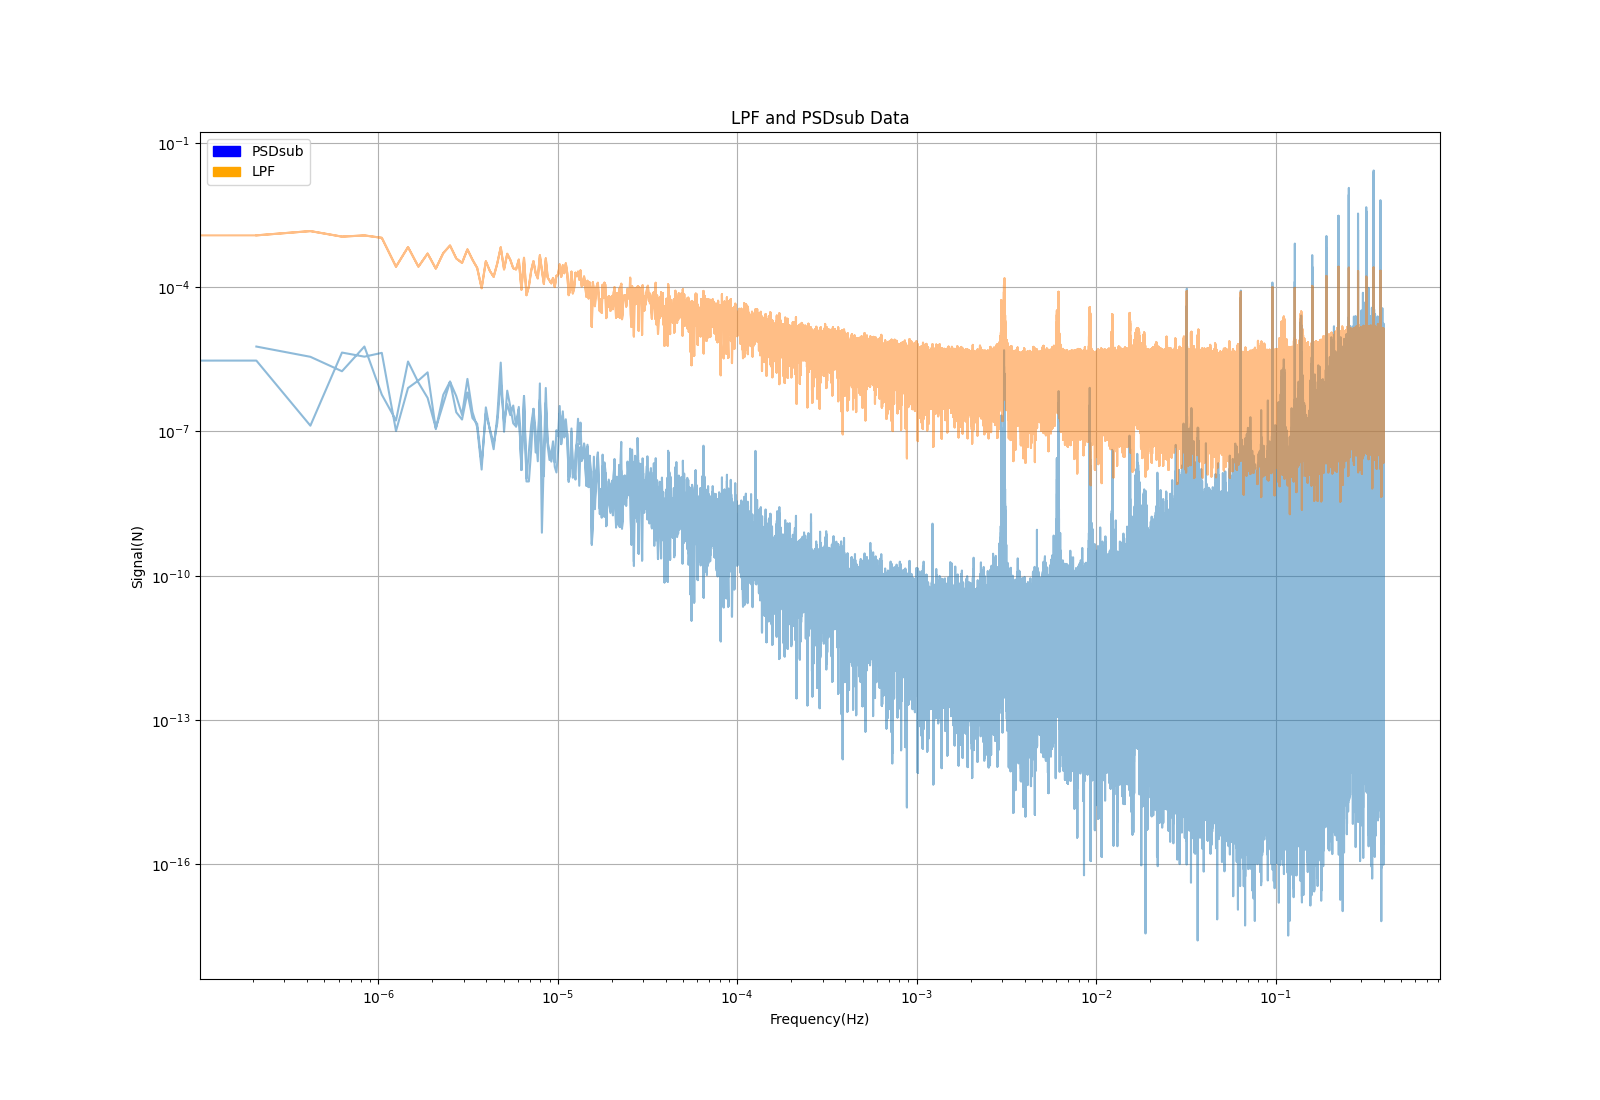
\includegraphics[width=0.5\textwidth]{LPF_Noise_Cancellation2.png}}
\caption{Noise cancellation plot of the original LPF data versus the original LPF data minus the spurious solar wind acceleration noise}
\label{fig}
\end{figure}
Figure 7 is a noise subtraction plot. Figure 6 displays the difference between the original LPF data and the LPF data that had the spurious solar wind acceleration noise removed. This plot is not completely accurate.\\

\section{Results}

\section{Conclusion}
The effects of spurious solar wind on acceleration noise of LPF data were found to be inconsequential. As shown in Figure z, the coherence between the ACE and LPF data was sporadic for the given frequency range. The lack of continual coherence proves that the LPF acceleration noise is not affected by spurious solar wind.  The lack of added acceleration noise will aid in the precision of the data gathering of LISA when the antenna launches.

%\begin{acknowledgments}
%\end{acknowledgments}


% The \nocite command causes all entries in a bibliography to be printed out
% whether or not they are actually referenced in the text. This is appropriate
% for the sample file to show the different styles of references, but authors
% most likely will not want to use it.
\nocite{*}

\bibliography{apssamp}% Produces the bibliography via BibTeX.

\end{document}
%
% ****** End of file apssamp.tex ******
e
